\documentclass[11pt]{article}

\usepackage[authoryear]{natbib}
\setlength{\bibsep}{6pt}
\usepackage[shortlabels]{enumitem} 
%\usepackage{hyperref}
\usepackage{caption}
\usepackage{geometry}
\usepackage{setspace}
\usepackage{float}
\usepackage{placeins}
\usepackage{amsmath}

\usepackage{amsthm}
\usepackage{comment}
\usepackage{amssymb}
\usepackage{graphicx}
\usepackage{amscd}
\usepackage{amsfonts}
\usepackage{epsfig}
\usepackage{framed}
\usepackage{asymptote}
\newtheorem{theorem}{Theorem}

% In case an author wants to include a very wide matrix.
\setcounter{MaxMatrixCols}{30}

% The following commands will set up the page geometry according to the default TRIUMPHS style.  Please modify them wisely, if at all.  As needed for a specific PSP, please address bad page and line breaks using commands such as \newpage and\or otherwise inserting/deleting space between lines.

\setlength{\topmargin}{-.7in}
\setlength{\oddsidemargin}{-.1in}
\setlength{\evensidemargin}{-.1in}
\setlength{\textwidth}{6.6in}
\setlength{\textheight}{9.3in}

\addtolength{\skip\footins}{10pt}
\linespread{1.1}

% The new command \sep defined here will produce the `extended infinity' symbol used to separate PSP narrative from primary source text within the `source' environment defined below.
\newcommand{\sep}{\vspace{-3pt}
\begin{center}
{\mathversion{normal}
$\infty \mspace{-5.5mu}\infty \mspace{-5.5mu}\infty \mspace{-5.5mu}\infty \mspace{-5.5mu}
\infty \mspace{-5.5mu}\infty \mspace{-5.5mu}\infty \mspace{-5.5mu}\infty \mspace{-5.5mu}
\infty \mspace{-5.5mu}\infty \mspace{-5.5mu}\infty \mspace{-5.5mu}\infty \mspace{-5.5mu}
\infty \mspace{-5.5mu}\infty \mspace{-5.5mu}\infty \mspace{-5.5mu}\infty \mspace{-5.5mu}
\infty \mspace{-5.5mu}\infty \mspace{-5.5mu}\infty \mspace{-5.5mu}\infty \mspace{-5.5mu}
\infty \mspace{-5.5mu}\infty \mspace{-5.5mu}\infty \mspace{-5.5mu}\infty \mspace{-5.5mu}
\infty \mspace{-5.5mu}\infty \mspace{-5.5mu}\infty \mspace{-5.5mu}\infty \mspace{-5.5mu}
\infty \mspace{-5.5mu}\infty \mspace{-5.5mu}\infty \mspace{-5.5mu}\infty \mspace{-5.5mu}
\infty \mspace{-5.5mu}\infty \mspace{-5.5mu}\infty \mspace{-5.5mu}\infty \mspace{-5.5mu}
\infty \mspace{-5.5mu}\infty \mspace{-5.5mu}\infty \mspace{-5.5mu}\infty \mspace{-5.5mu}$}
\end{center} \vspace*{-5pt}}

% This defines the environment for setting off primary source material with the `infinity' symbol before and after the source material. The source material itself will be set in a quote environment in sans serif font. For very short primary source excerpts, use your discretion concerning whether this environment makes sense, but please always use sans serif font (\sf) for primary source excerpts.

  \newenvironment{source}%
 {\bigskip \sep \vspace*{-6pt} \begin{quote}
          \begin{sf}   }
   {   \end{sf}     \end{quote} \vspace*{-6pt} \sep \bigskip}%

\newcounter{tasknumb}
\newcommand{\tasknumb}[1]{\refstepcounter{tasknumb}\textmd{\textbf{$\fbox{$\fbox{Task \thetasknumb}$}$}}#1}
\newcommand{\etc}{\text{etc.}}

%\setlist[1]{itemsep=50pt}

% This defines a new environment for student tasks.  A double box will be placed around 'Task xx', where the  number xx is updated with each new task.
\newenvironment{task}[1][]%
 {\begin{itemize}
 \item[\tasknumb{#1}]  }
{
    \end{itemize}    }%



%%%%%%%%%%%%%%%%%%%%%%%%%%%%%%%%%%%%%%%%%%%%%%%%%%%%%%%%%%%
\begin{document}


\title{Fourier's Proof of the Irrationality of $e$}
\author{Kenneth M Monks \thanks{Department of Mathematics, Front Range Community College -- Boulder County Campus, Longmont, CO 80537; \texttt{kenneth.monks@frontrange.edu}.
}}
\bigskip


\maketitle

\vspace*{-10pt}

We begin with a short passage from Aristotle's\footnote{Aristotle (384 BCE--322 BCE) was born in northern Greece.  His father, a doctor, wanted him to go into medicine.  However, both of Aristotle's parents passed when he was quite young, so he ended up enrolling at Plato's Academy in Athens at the age of seventeen.  There he received an education from Eudoxus (among others), whose work was incorporated into Euclid's \emph{Elements}, who was running the academy in Plato's absence. Aristotle eventually became a teacher at the academy, a position he held for twenty years \citep{StAndrewsAristotle}.} \emph{Prior Analytics}\footnote{Written or dictated by Aristotle in roughly 350 BCE, \emph{Prior Analytics} was most likely a collection of lecture notes.  It is today considered the first writing on pure logic, dealing largely with syllogisms and how statements about particulars can relate to statements about universals \citep{Aristotle}. It contains the now famous argument that goes as follows: every Greek is a person and every person is mortal, therefore every Greek is mortal.}. This translation was completed by Oxford scholars in 1931 and compiled by Richard McKeon into \emph{The Basic Works of Aristotle} \citep{Aristotle}.

\begin{source}
\S I.23.  For all who effect an argument \emph{per impossibile} infer syllogistically what is false, and prove the original conclusion hypothetically when something impossible results from the assumption of its contradictory; e.g.\ that the diagonal of a square is incommensurate with the side, because odd numbers are equal to evens if it is supposed to be commensurate.
\end{source}

The goal of this project is to work through a proof of the irrationality of the number $e$ due to Joseph Fourier.  This number would not have even been \emph{defined} in any publication for another two millennia\footnote{It was first formulated by Jakob Bernoulli in the context of compound interest in 1683 \citep{DSB}.} (plus a few years) after the writing of \emph{Prior Analytics}!  So, the reader may wonder why we are rewinding our clocks so far back.  Well, it turns out that the  key ideas required to understand Fourier's proof of the irrationality of $e$ can be traced right back to that passage from Aristotle. 

In Section \ref{contradiction}, we extract the key pattern of Aristotelian logic needed to understand Fourier's proof, and give it a bit more of a modern formulation.  In Section \ref{incommensurate}, we embark on a detailed exploration of the idea of two numbers being ``{\sf incommensurate}'', and then in Section \ref{numbers} we recast that idea in terms of important sets of numbers which have come to characterize so much of modern mathematics.  In Section \ref{e}, we examine Fourier's proof (as written by de Stainville) of the irrationality of $e$.  For a lovely epilogue (epi-natural-log?), we witness in Section \ref{eSquared} how Liouville extended Fourier's argument to learn a bit more about just how interesting a number $e$ is.

\section{Proof by Contradiction}\label{contradiction}

Let us revisit the Aristotle passage in slightly more bite-size pieces.  

\begin{source} For all who effect an argument \emph{per impossibile} infer syllogistically what is false, and prove the original conclusion hypothetically when something impossible results from the assumption of its contradictory\ldots 
\end{source}

For our purposes here, the phrase ``{\sf infer syllogistically}'' can be simply taken to mean that one concludes a statement from two or more prior statements. We can then analyze what the other items refer to.  We have the following: 
\begin{itemize}
    \item ``{\sf original conclusion,}'' meaning what is desired to be proven,
    \item ``{\sf its contradictory,}'' meaning the negation of what is desired to be proven, and
    \item ``{\sf what is false,}'' meaning some statement previously known to be false.
\end{itemize}

This process, by which one proves a statement by assuming its negation and then deducing a known falsehood, is today most commonly called ``proof by contradition''\footnote{Note that the translator's choice of words here, \emph{reductio per impossibile}, is one way to describe contradiction (having reduced one's hypothesis to an impossible conclusion). However, it is common today to instead call proof by contradiction by another of Aristotle's argument forms, namely \emph{reductio ad absurdum} (reducing one's hypothesis to an absurd conclusion).  The difference is subtle but sometimes incredibly important!}, and remains one of the most powerful tools in the mathematician's toolbox.  Let us digest this with an example.
 Sometimes before using a pattern of logic in a mathematical argument, it helps to see it applied in a nonmathematical setting.  Here we show an argument that is considered the birth of modern climate science, taken from none other than our guest of honor, Joseph Fourier, in his 1827 paper \emph{On the Temperatures of the Terrestrial Sphere and Interplanetary Space} (translated in  \citep{Pierrehumbert}).

\begin{source}
The Earth is heated by solar radiation\ldots Our solar system is located in a region of the universe of which all points have
a common and constant temperature, determined by the light rays and the heat sent by all the surrounding stars. This cold temperature of the interplanetary
sky is slightly below that of the Earth's polar regions.  The Earth would have
none other than this same temperature of the Sky, were it not for \ldots causes
which act \ldots to further heat it.
\end{source}

This very consequential passage is often cited today as the first proof of the existence of the greenhouse effect.  We claim this is an Aristotelian argument \emph{per impossibile}!  Or in modern terms, a proof by contradiction. 

\begin{task} In Fourier's argument above, which words play the roles of which parts in Aristotle's argument?  Specifically, find in Fourier's words the following components of an argument \emph{per impossibile}, as identified by Aristotle:
    \begin{itemize}
        \item ``{\sf original conclusion}'',
        \item ``{\sf its contradictory}'',
        \item ``{\sf [syllogistic inference]}'', and
        \item ``{\sf what is false}''.
    \end{itemize}
\end{task}

\section{Incommensurate Numbers}\label{incommensurate}

As we have seen, Aristotle's choice of example for a proof by contradiction involved the idea of ``{\sf incommensurate numbers}''.  In this section, we wish to elaborate upon what exactly that phrase means.

To the ancient Greeks, two quantities would be considered \emph{commensurate} if they could both be expressed as a whole number of multiples of the same length.  For example, the circumference of a circle of radius 2 and the circumference of a circle of radius 3 would be commensurate.  One could take the circumference of a circle of radius 1; the former would be twice that measurement and the latter would be three times that measurement.  Thus, the two quantities are commensurate (they can be measured together).  

Let us look at another example of commensurate lengths in a figure, to hopefully get a bit more of a feel for what that relation means.

\begin{task}
    Let $\triangle ABC$ be a triangle, let $D$ be the intersection of its three medians\footnote{Recall that a \emph{median} of a triangle is a segment that connects a vertex to the midpoint of the opposite side.}, and let $E$ be the midpoint of side $BC$. Explain why the lengths of $AE$ and $AD$ are commensurate.  ({\bf Hint:} There is a famous theorem from Euclidean geometry regarding the above configuration. However, if you do not recall it, or you did not encounter it on your mathematical path, perhaps begin by measuring $AE$ and $AD$ in some special cases, like the case where $\triangle ABC$ is an equilateral triangle or a right triangle. Then see if you can recall or look up the general theorem.)
\end{task}

We now revisit the final line in the Aristotle passage. 

\begin{source}
\ldots the diagonal of a square is incommensurate with the side, because odd numbers are equal to evens if it is supposed to be commensurate.
\end{source}

Aristotle does not give the details or intermediate steps of this argument; it is not obvious at all how the assumption of commensurability of the diagonal of the square with the side of the square results in an odd number equalling an even number.  However, his casual mention of it indicates that it was likely a well-known argument in his time, even though we have no written record of exactly what that argument was.  Here, we present one such possible argument, admittedly using more symbolic algebra than the Greeks had available to them at the time, but it will use the same essential ideas\footnote{For a slightly more complicated but purely geometric argument, see \citep[51]{Katz}.}. 

\begin{task}[\label{sqrt2}]
\begin{enumerate}[(a)]
    \item The \emph{common measure} of two lengths can be defined as the largest possible length that the two lengths are both integer multiples of.  For example, the common measure of a segment of length 9 and a segment of length 12 would be a segment of length 3, since the first is three times longer ($3\cdot 3=9$) and the second is four times longer ($4 \cdot 3=12$).  Explain why, given two quantities $a$ and $b$ having common measure $c$, at least one of the numbers $a/c$ and $b/c$ must be odd. 
    \item Let the points $A,B,C,D$ be the vertices of a square, labelled in clockwise order.  Let $d$ be the common measure of $AB$ (a side) and $AC$ (a diagonal).  Thus, $|AB|=d\cdot m$ for some whole number $m$ and $|AC|=d \cdot n$ for some whole number $n$.  Explain why one of $m$ or $n$ must be odd.
    \item Apply the Pythagorean Theorem to  $\triangle ABC$ to deduce that $2m^2=n^2$.  \item Explain why if $n$ is odd, then ``{\sf odd numbers are equal to evens}'', as Aristotle says.
    \item Explain why if $n$ is even and $m$ is odd, then again ``{\sf odd numbers are equal to evens}'', as Aristotle says.
    \item Explain why we do not need to consider the case where $n$ and $m$ are both even.
    \item To place the argument into proper form, clearly identify what the three key components are in this case:  ``{\sf original conclusion}'', ``{\sf its contradictory}'',
    and ``{\sf what is false}''.  In the end, what have we successfully demonstrated?
    \end{enumerate}
\end{task}

\section{Some Fundamental Sets of Numbers}\label{numbers}

 Though by no means an exhaustive list, we now present a few fundamental sets of numbers\footnote{There are a great many more number systems mathematicians work with, for example quaternions and integers mod $n$. However, they do not come up in the primary sources we include in this project.}.  Mathematicians use these particular number systems so frequently that there is a standard notation that has been adopted to refer to them, which we show below.
 
 \begin{itemize}
 \item {\bf Natural Numbers.} The set $\mathbb{N}$ of natural numbers is the set of all positive whole numbers, along with zero\footnote{Some mathematicians do not include zero in the set of natural numbers.  Here, we do.}.  That is, $$\mathbb{N}=\lbrace 0,1,2,3,4,5,\ldots \rbrace $$    
 \item {\bf Integers.} The set of integers $\mathbb{Z}$ is the set of all whole numbers, whether they are positive, negative, or zero.  That is, $$\mathbb{Z}=\lbrace \ldots,-4,-3,-2,-1,0,1,2,3,4,\ldots \rbrace $$ 
 
 \item {\bf Rational Numbers.} The set of rational numbers $\mathbb{Q}$ is the set of all numbers expressible as a fraction whose numerator and denominator are both integers.  
 
 \item {\bf Real Numbers.} The set of real numbers $\mathbb{R}$ is the set of all numbers expressible as a decimal expansion (finite or infinite).

\item {\bf Complex Numbers.} The set $\mathbb{C}$ of complex numbers is the set of all numbers expressible as $a+bi$, where $a$ and $b$ are real numbers, and $i$ is a symbol such that $i^2=-1$.  
 \end{itemize}
 
The figure below illustrates the relationships among these number systems, each labelled with the corresponding blackboard bold letter\footnote{If one wants an easy way to remember this notation: we have simply $\mathbb{N}$ for \underline{N}atural, $\mathbb{R}$ for \underline{R}eal, and $\mathbb{C}$ for \underline{C}omplex.  The two that don't seem to match their leading letter also have good reasons for their naming: $\mathbb{Z}$ for \underline{Z}ahl, which is German for ``number'', and $\mathbb{Q}$ for \underline{Q}uotient.}, along with a few examples from each set of numbers.  Note the inclusion of each number system in the next: every natural number is also an integer, every integer is rational, and so on.  For example, the number 2 is in the set of complex numbers because the set of complex numbers contains all of the other sets shown here. 
 
\begin{center}
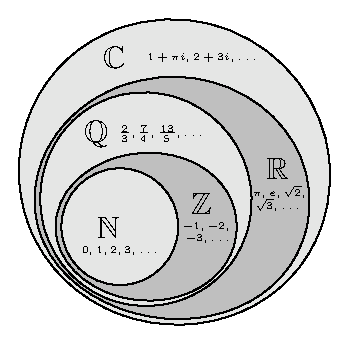
\includegraphics[scale=2]{NumberNotation.eps}
\end{center}
 
We define one last term before proceeding. 

\begin{itemize}
    \item 
A  number is called \emph{irrational} if it is real but not rational.  That is, $r$ is irrational if and only if $r\in\mathbb{R}$ but $r\not \in \mathbb{Q}$.
\end{itemize}

More visually, we are trying to identify what numbers lie outside the region marked with $\mathbb{Q}$ but inside the region marked with $\mathbb{R}$ in the diagram above.  Such numbers are called \emph{irrational}, and the diagram shows a few famous ones: $\pi, e, \sqrt{2},$ and $\sqrt{3}.$  

\begin{task}
\begin{enumerate}[(a)]
    \item What does the discussion above have to do with numbers being incommensurate?  Explain why a number is \emph{rational} if and only if it is commensurate with an integer\footnote{If you have had a course in discrete mathematics, you may have seen the notion of \emph{equivalence relation} and \emph{equivalence class}.  In that case, you may reinterpret this task as the following slightly stronger statement: prove that ``commensurate'' is an equivalence relation, and that the set of rational numbers is the equivalence class of 1.  If you have not yet had a course in discrete mathematics, revisit this footnote once you do!}.
    \item Set $|AB|=1$ in Task \ref{sqrt2}.  What does that imply the length $|AC|$ equals?
    \item Use the results of Task \ref{sqrt2} along with your work in this task to explain why $\sqrt{2}$ is irrational.
    \end{enumerate}
\end{task}
Thus, using a \emph{per impossibile} argument, we have verified that $\sqrt{2}$ really does belong in the part of the diagram in which it was placed! 

% \subsection{Proving Numbers are Rational}

% Recall that the set of rational numbers is the set of all numbers that can be expressed as the ratio of two integers.  More formally, 

% $$ {\mathbb{Q}}= \Bigg \lbrace \frac{a}{b} : a, b \in { \mathbb{Z} }, b \not = 0 \Bigg \rbrace. $$  So, to show a number $q$ is rational is usually not terribly hard. We simply need to find integers $a$ and $b$ such that their ratio is $q$.

% \begin{task}{Definition of Rational Numbers  }
% Show that the real number 2.1 is rational.  What is your $a$ and what is your $b$?
% \vspace*{0.1in}

% \end{task}

% If the decimal expansion is repeating and not terminating, it is slightly more tricky, as we need an infinite geometric series.  
% \begin{task}{Repeating Decimals are Rational    }
% \begin{itemize}
% \item Use a geometric series to show the number $0.0131313131313\ldots$ is rational.  What is your $a$ and what is your $b$?

% \item Let us generalize the example above.  We can use the infinite geometric series formula to prove that every number with a repeating decimal expansion is rational.  Specifically, assume you start with a repeating decimal and evaluate it using the infinite geometric series formula.  Explain why the numbers being plugged into the geometric series formula will all be rational as well as the output from that formula.

% \vspace{0.25in}

% \end{itemize}
% \end{task}

More generally, in order to use proof by contradiction to show that a real number $r$ is irrational, one can perform the following steps:

\begin{enumerate}
\item Assume $r$ is rational.
\item Thus, there must exist some integers $m$ and $n$ with $r=\frac{m}{n}$.
\item Use the equation $r=\frac{m}{n}$ and known properties of the number $r$ to deduce a statement we know is false. 
\item Conclude that our assumption of $r$ being rational must have been false, so $r$ is in fact irrational.
\end{enumerate}

\begin{task}\begin{enumerate}[(a)]
    \item Take the argument for the irrationality of $\sqrt{2}$ and adapt it to write a proof of the irrationality of $\sqrt{3}$.
    \item Suppose you try to adapt it to prove the irrationality of $\sqrt{4}$.  Where does the argument break down?
\end{enumerate}

\end{task}
\section{Fourier's Proof of the Irrationality of $e$}\label{e}

Joseph Fourier (1768--1830) was born into a working-class family in Auxerre, France. He quickly entered unfortunate circumstances: at the age of eight he became an orphan.  Luckily, he obtained admission to a local military school, where he received an education from the Benedictine monks of Saint-Maur.  In 1790, they gave him a mathematics teaching appointment at their school in Auxerre, where he also taught rhetoric, history, and philosophy.  He later became a founding faculty member at the \`{E}cole Polytechnique in Paris, where Napoleon sometimes attended lectures.  This led to Napoleon's request for Fourier's help in the administration of Egypt after its occupation by France in 1798.  Upon his return to France, Fourier served as the prefect of the Department of Is\`{e}re, where he led extensive infrastructure projects to quell chronic infections that were emanating from marshes in the area.  In 1817, he was elected to the Acad\'emie des Sciences, and five years later he became their perpetual secretary.  (For more on Fourier's life, see \citep{GreatBooks}.)  

Thus, Fourier was quite the busy person, not only as an academic but also as a civil servant.  Perhaps then, it is not terribly surprising that Fourier himself never wrote out and published his proof that $e$ is irrational!  Rather, it appears in the book \emph{M\'{e}langes d'analyse alg\'{e}brique et de g\'{e}om\'{e}trie} \citep[339]{Stainville} (\emph{Mixtures of algebraic analysis and geometry}) by Janot de Stainville\footnote{Nicolas Dominique Marie Janot de Stainville was a member of the \'Ecole Polytechnique class of 1802.  He was then hired back by his alma mater to work as a tutor in 1810 \citep{Verdier}.}  (1783--1828), who explained how the proof was communicated to him. 

\begin{source}
Note: this demonstration has been shared with me by Mr.\ Poinsot, who had it from Mr.\ Fourier.
\end{source}

The ``{\sf Mr. Poinsot}'' he refers to is Louis Poinsot\footnote{Louis Poinsot was a student and then later a professor at \'Ecole Polytechnique in Paris. He is perhaps best remembered for having written \emph{El\'ements de statique}, which is today considered to be the founding work on geometric mechanics.} (1777--1859). Poinsot and Fourier share a particular honor: they are both included among the seventy-two names of prominent mathematicians and scientists engraved into the Eiffel Tower!  Let us now walk through this proof together.\footnote{Note that we are reproducing the original notation symbol for symbol.  The lower dots are used to indicate multiplication.  For example, de Stainville uses $1.2$ to represent ``1 times 2'' rather than a decimal form of six-fifths.  Furthermore, note that de Stainville's order of operations had the lower dot evaluated \emph{after} addition, which is the opposite of what we typically do with multiplication vs addition.}

\begin{source}
After having found an approximate value for the number $e$, it is good to consider it in itself, and to demonstrate that not only is it comprised between $2$ and $3$, but that no rational fraction comprised between these two numbers can represent it; first it is greater than $2$, because the two first terms of the series
$$1+1+\frac{1}{2}+\frac{1}{2.3}+\frac{1}{2.3.4}+\text{etc.}, $$ are both equal to one, and the sum of the other terms is positive, but this sum is less than the sum of the terms of the equation $$\frac{1}{2}+\frac{1}{2^2}+\frac{1}{2^3}+\text{etc.},$$ which is equal to one, because it derives from the division of $1$ by $2-1$, it follows that the sum of the fractions $$\frac{1}{2}+\frac{1}{2.3}+\frac{1}{2.3.4}+\text{etc.}, $$ is necessarily less than one, and thus, that the number $e$ is lesser than 3.
\end{source}

\begin{task}
Although this is a very nicely written argument, a few steps could benefit from more detail.  To this end, explain carefully why each of the following claims is true: 
\begin{enumerate}[(a)]
    \item ``{\sf this sum is less than the sum of the terms of the equation}''  
    \item ``{\sf because it derives from the division of $1$ by $2-1$.}'' (In particular, be sure to identify which famous formula is being applied on that step!)
     
    \item ``{\sf the number is less than $3$.}''
\end{enumerate}
\end{task}

Having established that $e$ is in fact some real number between $2$ and $3$, de Stainville moved on to present Fourier's proof of irrationality\footnote{Notice that de Stainville's argument that $2<e<3$ and Fourier's proof of the irrationality of $e$ have something in common: they both depend on the formula $e=\sum_{n=0}^\infty \frac{1}{n!}$. This formula was due to the exceptionally talented and indescribably influential Swiss mathematician Leonhard Euler (1707--1783).  Be aware that there are plenty of other ways to define $e$, however. Jakob Bernoulli (1655--1705) gave the first construction of the number as $e=\lim_{n\to \infty}\left(1+\frac{1}{n}\right)^n$ in the context of studying compounded interest.  Euler initially defined $e$ to be the number that satisfied the special limit $\lim_{h\to 0 }\frac{e^h-1}{h}=1$ as he was looking for a nice base for calculating logarithms (see \citep{Ruch} for a PSP that guides the reader through Euler's paper which demonstrated the equivalence of the three definitions stated above).  Euler gave other characterizations of $e$, including continued fraction expansions relating to solutions of Ricatti differential equations, which he used to prove the irrationality of $e$ (see the article \emph{Who proved $e$ is irrational?} \citep{Sandifer} for a guided tour of Euler's work on this). }.

\begin{source}
I also affirm that no rational fraction can represent it, because if an irreducible fraction $m/n$ was equal to it, we would have $$\frac{m}{n}=2+\frac{1}{2}+\frac{1}{2.3}+\cdots+\frac{1}{2..n}+\frac{1}{2..n.n+1}+\text{etc.};$$ but if we multiply the two sections of this equation by the multiplication $1.2..n$ of the set of natural numbers, until the one that indicates the denominator of the fraction that lies in the first section, we will have 

$$\lbrace 1.2\ldots n-1 \rbrace m = \text{ an integer } + \frac{1}{n+1}+ \frac{1}{n+1.n+2}+\frac{1}{n+1.n+2.n+3}+\text{etc.},$$ or 
$$\frac{1}{n+1}+ \frac{1}{n+1.n+2}+\frac{1}{n+1.n+2.n+3}+\text{etc.}$$ is smaller than 
$$\frac{1}{n+1}+ \frac{1}{(n+1)^2}+\frac{1}{(n+1)^3}+\text{etc.},$$ and since this last quantity is equal to $$\frac{1}{(n+1)-1},$$ and that the first member is a whole number, it follows that to a whole number one would add a fraction lesser than $1/n$, the result would be a whole number, which is absurd; and thus it is equally absurd to suppose that the number $e$ would be rational, and thus it is irrational. 

\end{source}

Let us process this proof by rewriting it in a more modern form, updating our language and notation a bit.  

\begin{task}

Fill in the missing parts of the proof that $e$ is irrational.  The blanks are labelled (a),(b),\ldots , (m).
\vspace*{.2in}

\begin{proof} First let's write $e$ as an infinite series.  To do this, recall the power series for the exponential function:  $$ e^x = \underline{\hspace*{.2in}(a)\hspace*{.2in}}$$ Set $x=1$ to get an infinite series expression for the number $e$: $$ e=e^1= \underline{\hspace*{.2in}(b)\hspace*{.2in}}$$

We proceed by using the classic proof technique called \underline{\hspace*{.2in}(c)\hspace*{.2in}}. Accordingly, we assume $e$ is rational and then show that it leads to an impossible statement.

Proceeding, we assume $e$ is rational.  Then, there exist some $m,n \in \mathbb{N}$, with $n>1$, such that

$$ e = \underline{\hspace*{.2in}(d)\hspace*{.2in}} $$

We now identify the statement that will produce our contradiction.  We will prove both of the following:

\begin{enumerate}
    \item The quantity $\frac{1}{n+1}+\frac{1}{(n+1)(n+2)}+\frac{1}{(n+1)(n+2)(n+3)}+\cdots$ {\bf is} an integer.
    \item The quantity $\frac{1}{n+1}+\frac{1}{(n+1)(n+2)}+\frac{1}{(n+1)(n+2)(n+3)}+\cdots$ {\bf is not} an integer.
\end{enumerate}

The first statement is demonstrated as follows.  We multiply both sides of the above equation by \underline{\hspace*{.2in}(e)\hspace*{.2in}} to obtain $$ n!e=(n-1)!m.  $$  Notice that the right-hand side is an integer because $\underline{\hspace*{.2in}(f)\hspace*{.2in}}$.  Thus, the left-hand side, $n!e$, must also be an integer.  Notice however, the left-hand-side can be decomposed as follows by substituting the infinite series for $e$ and applying the distributive law:

\begin{align*} n!e&=n!\left( 1+\frac{1}{1!}+\frac{1}{2!}+\cdots +\frac{1}{n!}+\frac{1}{(n+1)!}+\cdots \right) \\
&=n!\left( 1+\frac{1}{1!}+\frac{1}{2!}+\cdots +\frac{1}{n!}\right) + n!\left(\frac{1}{(n+1)!} +\frac{1}{(n+2)!}+\frac{1}{(n+3)!}+\cdots\right).\end{align*} The first term, $n!\left( 1+\frac{1}{1!}+\frac{1}{2!}+\cdots +\frac{1}{n!}\right),$ is an integer because $\underline{\hspace*{.2in}(g)\hspace*{.2in}}$.  Subtracting that term from both sides, we can rewrite the above equation as $$\frac{1}{n+1}+\frac{1}{(n+1)(n+2)}+\frac{1}{(n+1)(n+2)(n+3)}+\cdots = n!e - n!\left( 1+\frac{1}{1!}+\frac{1}{2!}+\cdots +\frac{1}{n!}\right). $$


\vspace{.1in}

We now proceed to show the second statement: that the quantity of interest is not an integer.  In particular, we will show that  $\left( \frac{1}{n+1}+ \frac{1}{(n+1)(n+2)}+\frac{1}{(n+1)(n+2)(n+3)}+\cdots\right)$ lies between $\frac{1}{n+1}$ and 
$\frac{1}{n}$.  However, there are no integers between $\frac{1}{n+1}$ and
$\frac{1}{n}$, since they are both between $0$ and $1$.  Proceeding, we have

\begin{align}
\frac{1}{n+1} &< \frac{1}{n+1}+ \frac{1}{(n+1)(n+2)}+\frac{1}{(n+1)(n+2)(n+3)}+\cdots \\
 &< \frac{1}{n+1}+ \frac{1}{(n+1)(n+1)}+\frac{1}{(n+1)(n+1)(n+1)}+\cdots \\
 &= \frac{1}{n+1}+ \frac{1}{(n+1)^2}+\frac{1}{(n+1)^3}+\cdots \\
 &= \frac{\frac{1}{n+1}}{1-\frac{1}{n+1}} \\
 &= \frac{1}{n}.
 \end{align} The above steps are justified as follows.  The inequality on line (1) is true because $\underline{\hspace*{.2in}(h)\hspace*{.2in}}$.  To get from line (1) to line (2), we use the fact that $\underline{\hspace*{.2in}(i)\hspace*{.2in}}$.  The link between line (2) and line (3) is simply algebra.  To get from line (3) to line (4), we sum an infinite geometric series with common ratio $\underline{\hspace*{.2in}(j)\hspace*{.2in}}$ and initial term $\underline{\hspace*{.2in}(k)\hspace*{.2in}}$.  The transition from line (4) to line (5) again follows from ordinary algebraic simplification.

Thus, we have demonstrated that $$ \frac{1}{n+1} <  \left( \frac{1}{n+1}+ \frac{1}{(n+1)(n+2)}+\frac{1}{(n+1)(n+2)(n+3)}+\cdots\right) < \frac{1}{n}, $$ as desired.  Since $\frac{1}{n+1}$ and $\frac{1}{n}$ are strictly between 0 and 1, the quantity $$\underline{\hspace*{.2in}(l)\hspace*{.2in}}$$ must lie strictly between 0 and 1 as well.  However, there are no integers between 0 and 1, so that quantity cannot be an integer.  

Thus, if our assumption that $e$ is rational were true, we would be able to prove the existence of a quantity that both is and is not an integer at the same time.  This is a contradiction.  Therefore, we conclude that $$\underline{\hspace*{1.25in}(m)\hspace*{1.25in}}.$$
\end{proof}
\end{task}

After reading a long and complicated argument, some small ``sanity check'' kind of questions are often helpful with regards to moving the argument from a place of ``I didn't disagree with that at any particular step'' to the much better place of ``ok, that argument feels intuitive to me''.  The following tasks hopefully help with that!

\begin{task}
First, let's make sure we understand the logic of the above argument. 
\begin{enumerate}[(a)]
\item Identify Aristotle's key components in this argument.  Specifically, identify each of the ``{\sf original conclusion}'', ``{\sf its contradictory}'',
    and``{\sf what is false}''?  At the end of all of this work, what have we successfully demonstrated?
    \item The contradiction was established by using the assumption of the rationality of $e$ to prove two statements (labelled ``1.'' and ``2.'' in the proof) that were in direct opposition to each other.  Which one was actually true? 
    \end{enumerate}
\end{task}

\begin{task} To help visualize what exactly happened in the argument above, plot the following five quantities in order on a number line: $0,1, \frac{1}{n}, \frac{1}{n+1}, $ and $\frac{1}{n+1}+ \frac{1}{(n+1)(n+2)}+\frac{1}{(n+1)(n+2)(n+3)}+\cdots$. 

\end{task}

\begin{task}
Why can we assume that $n>1$?  ({\bf Hint:} Revisit the first primary source passage from de Stainville!)  Furthermore, why was that important?  Where was that fact used in the proof?
\end{task}


\section{What about $e^2$?}\label{eSquared}

In his paper \emph{Sur l'irrationalite\'{e} du nombre $e=2,718\ldots$}, Joseph Liouville\footnote{Liouville's father, like Fourier, had worked with Napoleon during wartime. Liouville began study at the \'{E}cole Polytechnique in Paris in 1825. Upon graduating, he went on to become an enormously consequential mathematician with regards to the study of transcendental numbers.  Liouville considered the number $0.110001000000000000000001000\ldots$ that has a $1$ in any position given by $n!$ for some natural number $n$, and $0$ otherwise. He proved this number was transcendental in the landmark paper \emph{Sur les classes tr\`es \'etendues de quantit\'es dont la valeur n'est ni alg\'ebrique ni m\^me r\'eductible \`a des irrationelles alg\'ebriques} \citep{transcendental}.} (1809--1882) adapted Fourier's methods to prove that $e^2$ is also irrational.  We trace through his argument here.

\begin{source}

We will prove that the number $e$, the base of Napierian\footnote{This refers to what is today usually called ``natural log''.  This adjective is being applied in honor of its inventor, John Napier (1550--1617), a Scottish mathematician and physicist.} logarithms, isn't a rational value.  One should add, it seems to me, that the same method also proves that $e$ can't be the root of a second degree equation with rational coefficients, which means that one could not have $$ae+b/e=c,$$ $a$ being a whole positive number and $b,c$ whole numbers, positive or negative. 

Indeed, if we replace in this equation $e$ and $1/e$ or $e^{-1}$ by their expansions deduced from the expansion of $e^x$, since we multiply the two numbers by $1.2.3\ldots n,$ we will easily find $$\frac{a}{n+1}\left(1+\frac{1}{n+2}+\cdots \right)\pm \frac{b}{n+1}\left(1-\frac{1}{n+2}+\cdots \right)=\mu,  $$ $\mu$ being a whole number.  One can always make it so that the factor $$\pm \frac{b}{n+1}$$ is positive; it will suffice to assume $n$ is even if $b$ is $<0$ and $n$ is odd if $b$ is $>0$; by taking $n$ as very large, the equation that we just wrote is absurd; because its first section is essentially positive and very small, will be comprised between $0$ and $1$, and can't be equal to a whole $\mu$.  Thus, etc.

\end{source}



\begin{task}
 In Liouville's proof above, he never wrote out any representation of the number $e^2$ itself.  Why does his argument truly prove that quantity is irrational as claimed?  ({\bf Hint:} Take the equation  $ae+b/e=c$ from the above passage and multiply both sides by $e$.)
\end{task}

\begin{task}  Quite a bit of work is hidden in the early parts of this argument, as well as in Liouville's claim that the ``{\sf first section is essentially positive and very small}'' and thus ``{\sf will be comprised between 0 and 1}''.  Let us fill in some details in that claim.
\begin{enumerate}[(a)]
    \item Start with the infinite series expansions for both $e$ and $e^{-1}$.  Substitute them into the equation $ae+b/e=c$, and show the algebra needed to reach the statement $$ \frac{a}{n+1}\left(1+\frac{1}{n+2}+\cdots \right)\pm \frac{b}{n+1}\left(1-\frac{1}{n+2}+\cdots \right)=\mu.$$  What terms had to be pushed to the right-hand side to be part of the integer $\mu$?
    \item Write out the equation for $n=3$ and $n=4$.  In these examples, can you verify the claim that ``{\sf $n$ is even if $b$ is $<0$ and $n$ is odd if $b$ is $>0$}'' in these two specific cases?  Does it make sense that this would generalize to any $n$?  Explain why or why not.
    \item We now focus on the expressions $$\left(1+\frac{1}{n+2}+\cdots \right)$$ and $$\left(1-\frac{1}{n+2}+\cdots \right).$$  Liouville was perhaps a bit terse in only include two terms in each!  Write out these series again but show four terms in each instead of just two, just to make sure we see the general pattern.
    \item In de Stainville's writeup of Fourier's proof of the irrationality of $e$, he uses a comparison with a geometric series to show that $$\frac{1}{n+1}+\frac{1}{(n+1)(n+2)}+\frac{1}{(n+1)(n+2)(n+3)}+\cdots < 1/n.$$  Use a similar argument to show that $$\left(1+\frac{1}{n+2}+\cdots \right)<2$$ for all $n>1.$
    \item Conclude that the same upper bound holds for the magnitude of the corresponding alternating series.  That is, $$\left| \left(1-\frac{1}{n+2}+\cdots \right)\right|<2$$ as well.
    \item Explain why Liouville's claim that the expression $$\frac{a}{n+1}\left(1+\frac{1}{n+2}+\cdots \right)\pm \frac{b}{n+1}\left(1-\frac{1}{n+2}+\cdots \right)$$  ``{\sf will be comprised between 0 and 1}'' is true as long as $n$ is chosen to be at least $2a+2|b|$.
\end{enumerate}
\end{task}

\begin{task}
Once again, to be certain we understand the logic of the argument given above, identify Aristotle's key components.  Specifically, what are the ``{\sf original conclusion}'', ``{\sf its contradictory}'',
    and``{\sf what is false}'' in this argument?  In the end, what has Liouville successfully demonstrated?
\end{task}

We now compare two numbers whose irrationality we demonstrated in this project: $e$ and $\sqrt{2}$. 

\begin{task}
In a sense, $e$ is somehow \emph{more} irrational than $\sqrt{2}$.  In particular,\ldots
\begin{enumerate}[(a)]
\item \ldots if you square $\sqrt{2},$ do you get a rational number?  Why or why not?
\item \ldots if you square $e$, do you get a rational number?  Why or why not?
\end{enumerate}
\end{task}

The above observation starts to hint at the idea of a \emph{transcendental number}: a number that cannot be obtained as a root of a polynomial with integer coefficients.  While the square root of 2 is certainly irrational, it is a root of a polynomial with integer coefficients, namely $x^2-2.$  However, it turns out that $e$ is in fact transcendental as well as irrational.  This fact is much more difficult to prove than the irrationality of $e$.  Liouville in fact attempted this but never succeeded!  It was proven almost thirty years after $e$'s irrationality was published, by Charles Hermite\footnote{Charles Hermite was born in Dieuze, Lorraine, France. He became known not only for his contributions to number theory, analysis, linear algebra, and differential equations, but also for his spectacular teaching! \citep{HermiteBio} } (1822--1901) \citep{Hermite}.  Though the argument proved more difficult, it had something in common with all the arguments in this PSP: Hermite's proof still proceeded \emph{per impossibile}!

\vspace{0.1in}

\noindent\hrulefill

%\nocite{*}% This command is needed to ensure all bib items are listed in references, and not just those directly cited in the project.
 \bibliographystyle{plainnat}
      \bibliography{FourierProof}{}                              
      \pagebreak 
      
      
\section*{Notes to Instructors}

\subsection*{PSP Content: Topics and Goals}

This Primary Source Project (PSP) is intended to show students how the methods of series and their analysis are not only useful for Computation, but also for proving theoretical results. The key competencies that come up in this project are as follows:
\begin{itemize}
    \item Power series for $e^x$
    \item Infinite geometric series formula
    \item Comparison test arguments
\end{itemize}


\subsection*{Student Prerequisites}

In this project, we assume the student has already seen the standard treatments of the three topics listed above.
    
\subsection*{PSP Design, and Task Commentary}

This PSP will expose the student to arguments that extensively use the power series for $e^x$ and geometric series, but in the context of proofs of the irrationality of certain numbers.  This serves as a fabulous warm-up for a student who later takes an introduction to proof course; all arguments in this PSP use proof by contradiction.


\subsection*{Suggestions for Classroom Implementation}

Instructors are strongly encouraged to work the entire PSP before using it in class:  although only simple techniques are employed, the proofs are a bit subtle!


If one wishes to shorten the PSP, one could delete Section \ref{eSquared} entirely (though it is very fun).  Finishing with Section \ref{e} still tells a perfectly complete story in and of itself!  Section \ref{eSquared} is also a bit more challenging; one reasonable implementation would be to require the completion of the PSP through Section \ref{e} for the whole class, but then use Section \ref{eSquared} as an option for extra credit.    

 Copies of these PSPs are available at the TRIUMPHS website (see URL in Acknowledgements).  
The author is happy to provide \LaTeX\ code for this project.  It was created using Overleaf which makes it convenient to copy and share projects and can allow instructors to adapt this project in whole or in part as they like for their course.


\subsection*{Sample Implementation Schedule (based on a 50-minute class period)}

The author recommends two full 50-minute class periods for implementation of this PSP.
\begin{itemize}
    \item The readings and tasks of the PSP up to and including Section \ref{numbers} can be assigned as preparation for class.
    \item Start class with 20 minutes of followup discussion on the first two sections.  In particular, make sure the students are clear on all vocabulary involved.
    \item The next 30 minutes could consist of students working in small groups, working to understand the argument in Section 4. 
    \item During the first 20 minutes of the following class, the instructor could have students present solutions to the Section 4 argument and make sure everyone really understands it.  
    \item The remainder of the second class can be devoted to Section 5, with its completion assigned for homework.
\end{itemize}
 

 \vspace*{-3pt}
\subsection*{Connections to other Primary Source Projects}

 \vspace*{-3pt}
 
 
The following additional projects based on primary sources are also freely available for use in teaching standard topics in the calculus sequence. The PSP author name of each is given (together with the general content focus, if this is not explicitly given in the project title). With the exception of the final project in the list (which requires up to 2 full weeks for implementation), each of these is a mini-PSP that can be completed in 1--2 class days. Classroom-ready versions of these projects can be downloaded from  {\tt  https://digitalcommons.ursinus.edu/triumphs\_calculus}.



%\emph{Calculus 1}

 % \vspace*{-8pt}

\begin{itemize}
\item  The Derivatives of the Sine and Cosine Functions, Dominic Klyve 


\item Fermat's Method for Finding Maxima and Minima, Kenneth M Monks
\item Beyond Riemann Sums: Fermat's Method of Integration, Dominic Klyve



\item How to Calculate $\pi$: Buffon's Needle (calculus version), Dominic Klyve (integration by parts)


  \item Gaussian Guesswork: Elliptic Integrals and Integration by Substitution, Janet  Barnett


\item Gaussian Guesswork: Polar Coordinates, Arc Length and the Lemniscate Curve, Janet  Barnett

\item Gaussian Guesswork: Infinite Sequences and the Arithmetic-Geometric Mean, Janet  Barnett

\item Investigations Into d'Alembert's Definition of Limit (calculus version), Dave Ruch (sequence convergence)

\item How to Calculate $\pi$: Machin's Inverse Tangents, Dominic Klyve (infinite series)


 \item  Euler's Calculation of the Sum of the Reciprocals of Squares, Kenneth M Monks (infinite series)

 \item The Radius of Curvature According to Christiaan Huygens, Jerry Lodder
\end{itemize}

Another PSP that connects very nicely to this one is \emph{Euler's Rediscovery of $e$} by David Ruch \citep{Ruch}, which shows the origin of the infinite series for $e$ that Fourier's proof depends on.  Although that PSP is intended for use in an introductory course in analysis, it is quite appropriate for a second-semester calculus classroom if one simply stops at Task 5.

\subsection*{Recommendations for Further Reading}
Charles Hermite's paper \citep{Hermite}, in which $e$ is proven to be transcendental, would be a fabulous (though challenging) follow-up for the advanced student.

 \section*{Acknowledgments}
The development of this project has been partially supported by the Transforming Instruction in
Undergraduate Mathematics via Primary Historical Sources (TRIUMPHS) Project with funding
from the National Science Foundation's Improving Undergraduate STEM Education Program under Grants No. 1523494, 1523561, 1523747, 1523753, 1523898, 1524065, and 1524098. Any opinions, findings, and conclusions or recommendations expressed in this project are those of the author and do not necessarily reflect the views of the National Science Foundation.  The author would like to thank the TRIUMPHS PIs and Advisory Board for the very helpful feedback throughout the writing of this project.  

The author would especially like to thank two of his incredible former students: Diane Van Tiggelen, who provided translations for the French primary sources used in this PSP, and Jenna Allen, who created the number system diagram in Section \ref{numbers} in the context of creating a calculus OER together.

\bigskip
\bigskip
\begin{minipage}{.25\textwidth}
       \noindent
      
\includegraphics[scale=1]{by-sa.png}
 \end{minipage}%
 \begin{minipage}{0.7\textwidth}
       This work is licensed under a Creative Commons Attribution-ShareAlike 4.0 International License ({\tt https://creativecommons.org/licenses/by-sa/4.0/legalcode}). It allows re-distribution and re-use of a licensed work on the conditions that the creator is appropriately credited and that any derivative work is made available under ``the same, similar or a compatible license''.
\end{minipage}


\bigskip
\bigskip

\noindent For more information about the NSF-funded project TRansforming Instruction in Undergraduate Mathematics via Primary Historical Sources (TRIUMPHS), visit \\
{\tt http://blogs.ursinus.edu/triumphs/}.

\end{document}